% Gemini theme
% https://github.com/anishathalye/gemini
% We try to keep this Overleaf template in sync with the canonical source on
% GitHub, but it's recommended that you obtain the template directly from
% GitHub to ensure that you are using the latest version.

% Brown University color schemes for Gemini theme
% https://github.com/vskbellala/gemini-brown

\documentclass[final]{beamer}

% ====================
% Packages
% ====================

\usepackage[T1]{fontenc}
\usepackage{lmodern}
\usepackage[size=custom,width=120,height=72,scale=1.0]{beamerposter}
\usetheme{gemini}
\usecolortheme{brown}
% \usecolortheme{brownminimal}
\usepackage{graphicx}
\usepackage{amsmath, amssymb, amsfonts}
\usepackage{booktabs}
\usepackage[numbers]{natbib}  % numeric default
\bibliographystyle{plainnat}  % numeric, but keeps author-year info

\usepackage{tikz}
\usepackage{pgfplots}
\pgfplotsset{compat=1.14}

% ====================
% Lengths
% ====================

% If you have N columns, choose \sepwidth and \colwidth such that
% (N+1)*\sepwidth + N*\colwidth = \paperwidth
\newlength{\sepwidth}
\newlength{\colwidth}
\setlength{\sepwidth}{0.025\paperwidth}
\setlength{\colwidth}{0.3\paperwidth}

\setlength{\itemsep}{0.2em}
\setlength{\topsep}{0em}
\setlength{\parsep}{0em}

\newcommand{\tightlist}{\setlength\itemsep{0.2em}\setlength\topsep{0em}\setlength\parsep{0em}}

\newcommand{\separatorcolumn}{\begin{column}{\sepwidth}\end{column}}

% ====================
% Title
% ====================

\title{Investigating Determinants of Birth Weight Using Bayesian Tree-Based Nonparametric Modeling}

\author{Adam M. Kurth \inst{1} \and Richard P. Hahn \inst{2}}

\institute[shortinst]{\inst{1} Brown University, School of Public Health \samelineand \inst{2} Arizona State University}

% ====================
% Footer (optional)
% ====================

\footercontent{
    \href{https://adammkurth.netlify.app}{https://adammkurth.netlify.app} \hfill 
    JSM 2026, Boston, MA --- Poster ID: XYZ-1234 \hfill
    \href{mailto:adam_kurth@brown.edu}{adam\_kurth@brown.edu}}

% ====================
% Logo (optional)
% ====================

% use this to include logos on the left and/or right side of the header:
\logoright{
\includegraphics[height=7cm]{images/asu_somss.png}}
% \logoleft{
\includegraphics[height=7cm]{images/Brown_white.png}}
\logoleft{
\includegraphics[height=7cm]{images/Brown_full.png}}


% ====================
% Body
% ====================

\begin{document}

\begin{frame}[t]
\begin{columns}[t]
\separatorcolumn

\begin{column}{\colwidth}
\vspace{-1em}
\begin{block}{Introduction \& Motivation: Problem and Gaps}

    \textbf{Problem.} Low birth weight (LBW, \(\le\) 2.5 kg) is linked to elevated neonatal mortality and lifelong morbidity. Incidence reflects interacting socioeconomic, behavioral, and environmental factors. Public-health goal: identify \emph{interpretable} high-risk subgroups for targeted intervention. 

    \textbf{Gaps.}\vspace{-0.8em}
    \small
    \begin{enumerate}\tightlist
      \item Classical regression: additive form under-captures interactions.
      \item CART: interpretable, but impurity measures (e.g., Gini) ignore full BW distribution; suffers in sparse LBW tails.
      \item Bayesian density models: flexible but computationally intensive and opaque.
    \end{enumerate}

    \normalsize
    \textbf{Contribution.} DM-CART: combine CART's interpretability with Bayesian uncertainty by using Dirichlet-Multinomial (DM) \emph{marginal likelihood} as the splitting criterion. 
    
\end{block}


\begin{alertblock}{Dataset: Predictors and Coding}
    The 2021 Natality Data: 3.6 M birth records in all 50 states \cite{nber_birth_data}. 
    Seven predictor variables are chosen and retained based on clinical relevance and known associations with LBW incidence. Predictors are dichotomized into (1/0), yielding \(2^7 = 128\) predictor-class combinations.
    
    \vspace{-0.5em}
    \small
    \begin{table}[ht]
    \centering
    \small
    \setlength{\tabcolsep}{3pt}
    \caption{Binary predictor definitions}
    \begin{tabular}{@{}llll@{}}
    \toprule
    Label & Field & 1 = Yes & 0 = No \\ \midrule
    Boy          & sex      & Male  & Female \\
    Married      & dmar     & Married & Not married \\
    Black        & mrace15  & Black / African Am. & Other race \\
    Over33       & mager    & $>$33 yr & $\le$33 yr \\
    HighSchool   & medu     & HS completed & Otherwise \\
    FullPrenatal & prenatal & Adequate care & Inadequate/none \\
    Smoker       & cig\_0   & Any smoking & None \\
    \bottomrule
    \end{tabular}
    \end{table}

\end{alertblock}


\begin{block}{Binning \& Priors: Birth-Weight Categories and Dirichlet Parameters}

    Historic (2020) data define the decline-quantile cut-points in 10\% increments in the LBW range (0--2.5 kg), creating \textbf{Q1—Q10}, plus NBW (\(>2.5\)kg).

    \textbf{Matrices:} \(128 \times 11\) (full) and \(128 \times 10\) (LBW-only). \(K = \{10, 11\}\) depending on model.

    Dirichlet priors \(\boldsymbol{\alpha} = (\alpha_1, \dots, \alpha_K)\) from 2020 frequencies:\vspace{-0.8em}
    \begin{itemize}\tightlist
        \item Full model: NBW prior $\approx$91.67\%, LBW split across Q1–Q10.
        \item LBW-only: uniform 10\% per category.
    \end{itemize}
    
    \begin{minipage}{0.50\linewidth}
      \centering
      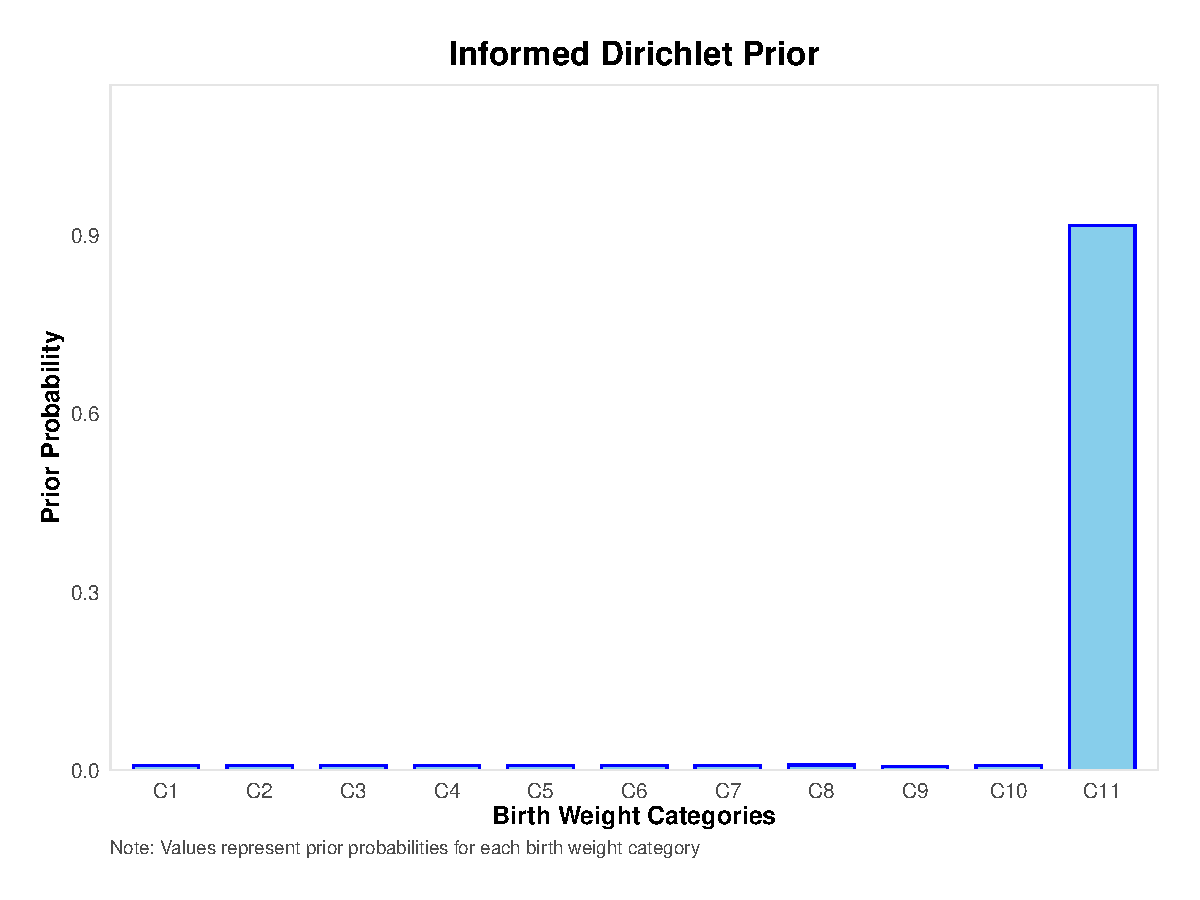
\includegraphics[width=\linewidth]{images/plots/alphavec_plot_2020_full.pdf}\\[-1ex]
      {\small Full model prior: LBW+NBW}
    \end{minipage}
    \hfill
    \begin{minipage}{0.50\linewidth}
      \centering
      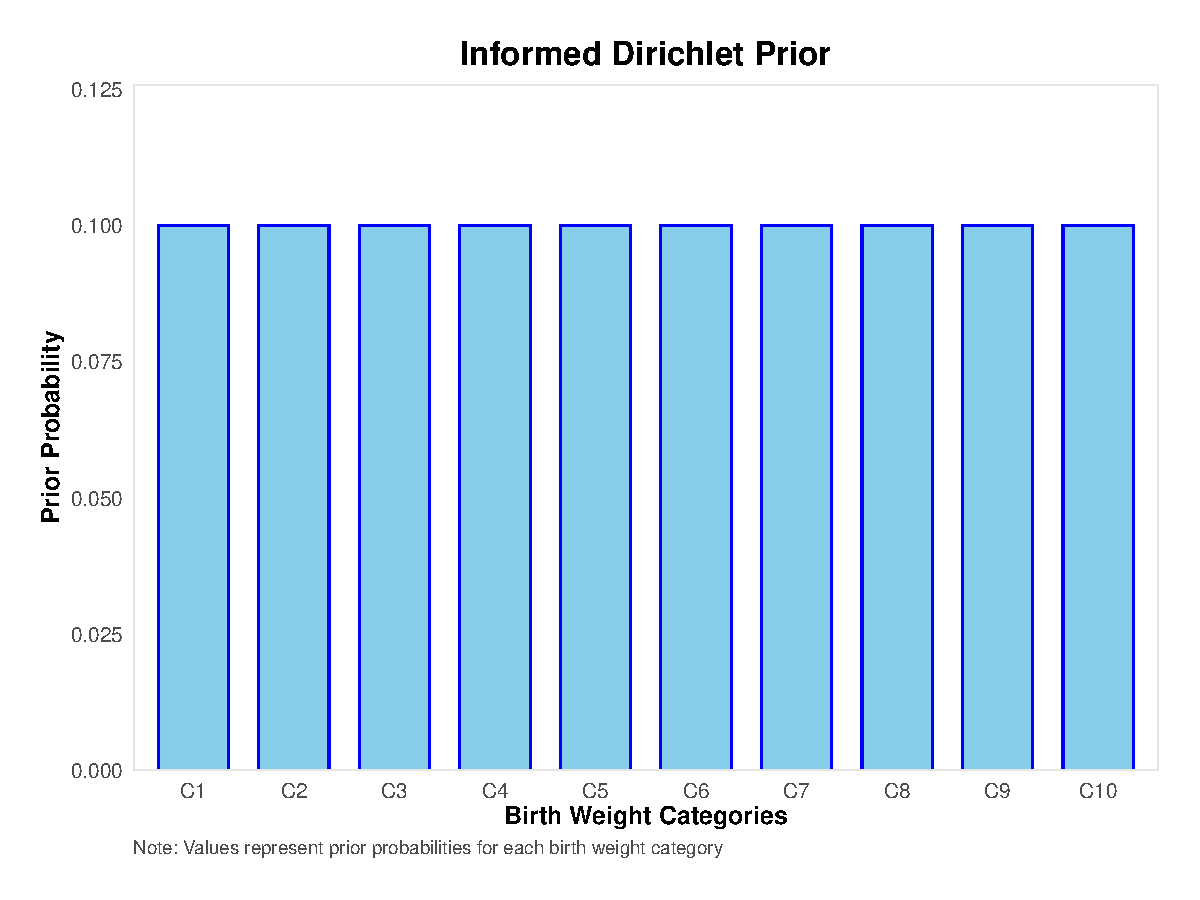
\includegraphics[width=\linewidth]{images/plots/alphavec_plot_2020_small.pdf}\\[-1ex]
      {\small LBW-only prior}
    \end{minipage}
    
\end{block}

\end{column}

\separatorcolumn

\begin{column}{\colwidth}
\vspace{-1em}
\begin{block}{DM–CART: Splitting Criterion and Likelihood}

    Predictor: \(\mathbf{X} \in \{0,1\}^{N \times 7}\) matrix and for profile \(i\), row \(\mathbf{x}_i \in \{0,1\}^7\) is fixed.  
    
    Response: \(\mathbf{Y} = \left[n_{i,k} \right]_{i=1}^N\) and for profile \(i\), row \(\mathbf{y}_i = (n_{i,1},\dots,n_{i,K})\) represent BW counts for \(K\) total BW categories. 

    \textbf{Hierarchical model:}
    \[
      \mathbf{y}_i \mid \boldsymbol{\theta}_i, \mathbf{x}_i \sim \mathrm{Multinomial}(N_i, \boldsymbol{\theta}_i), 
      \quad \boldsymbol{\theta}_i \mid \boldsymbol{\alpha} \sim \mathrm{Dirichlet}(\alpha_1,\dots,\alpha_K)
    \]
    
    where \(N_i = \sum_k n_{i,k}\), are the BW counts for profile \(i\), and \(\alpha_0 = \sum_k \alpha_k\) is constant.

    \small
    \emph{Note:} Multinomial coefficient \emph{omitted} due to data preprocessing and consolidation procedure.
    
    \normalsize
    \textbf{Node log-likelihood:}
    \[
    \ell_i = \log \Gamma(\alpha_0) - \log\Gamma(N_i + \alpha_0) + \sum_{k=1}^K\!\big[ \log\Gamma(n_{i,k}+\alpha_k) - \log\Gamma(\alpha_k) \big]
    \]

    \textbf{Split gain:} \(\Delta \ell = \ell_{\text{left}}+\ell_{\text{right}}-\ell_{\text{parent}}\). i.e. improvement in node homogeneity given split \citep{gundersen2020dirichlet-multinomial,mimno_polya,minka2000estimating}


    \textbf{Fitting:}\vspace{-0.6em}
    \small
    \begin{enumerate}\tightlist
      \item Evaluate all candidate splits via \(\Delta \ell\)
      \item Pick max positive split gain (improvement); recurse until depth limit or no-gain.
      \item Fit (i) full (NBW+LBW) and (ii) LBW-only models.
    \end{enumerate}
\end{block}

\vspace{-.3em}
\begin{alertblock}{Tree Structures: Full vs. LBW-Only Models}
    \begin{minipage}{0.50\linewidth}
      \centering
      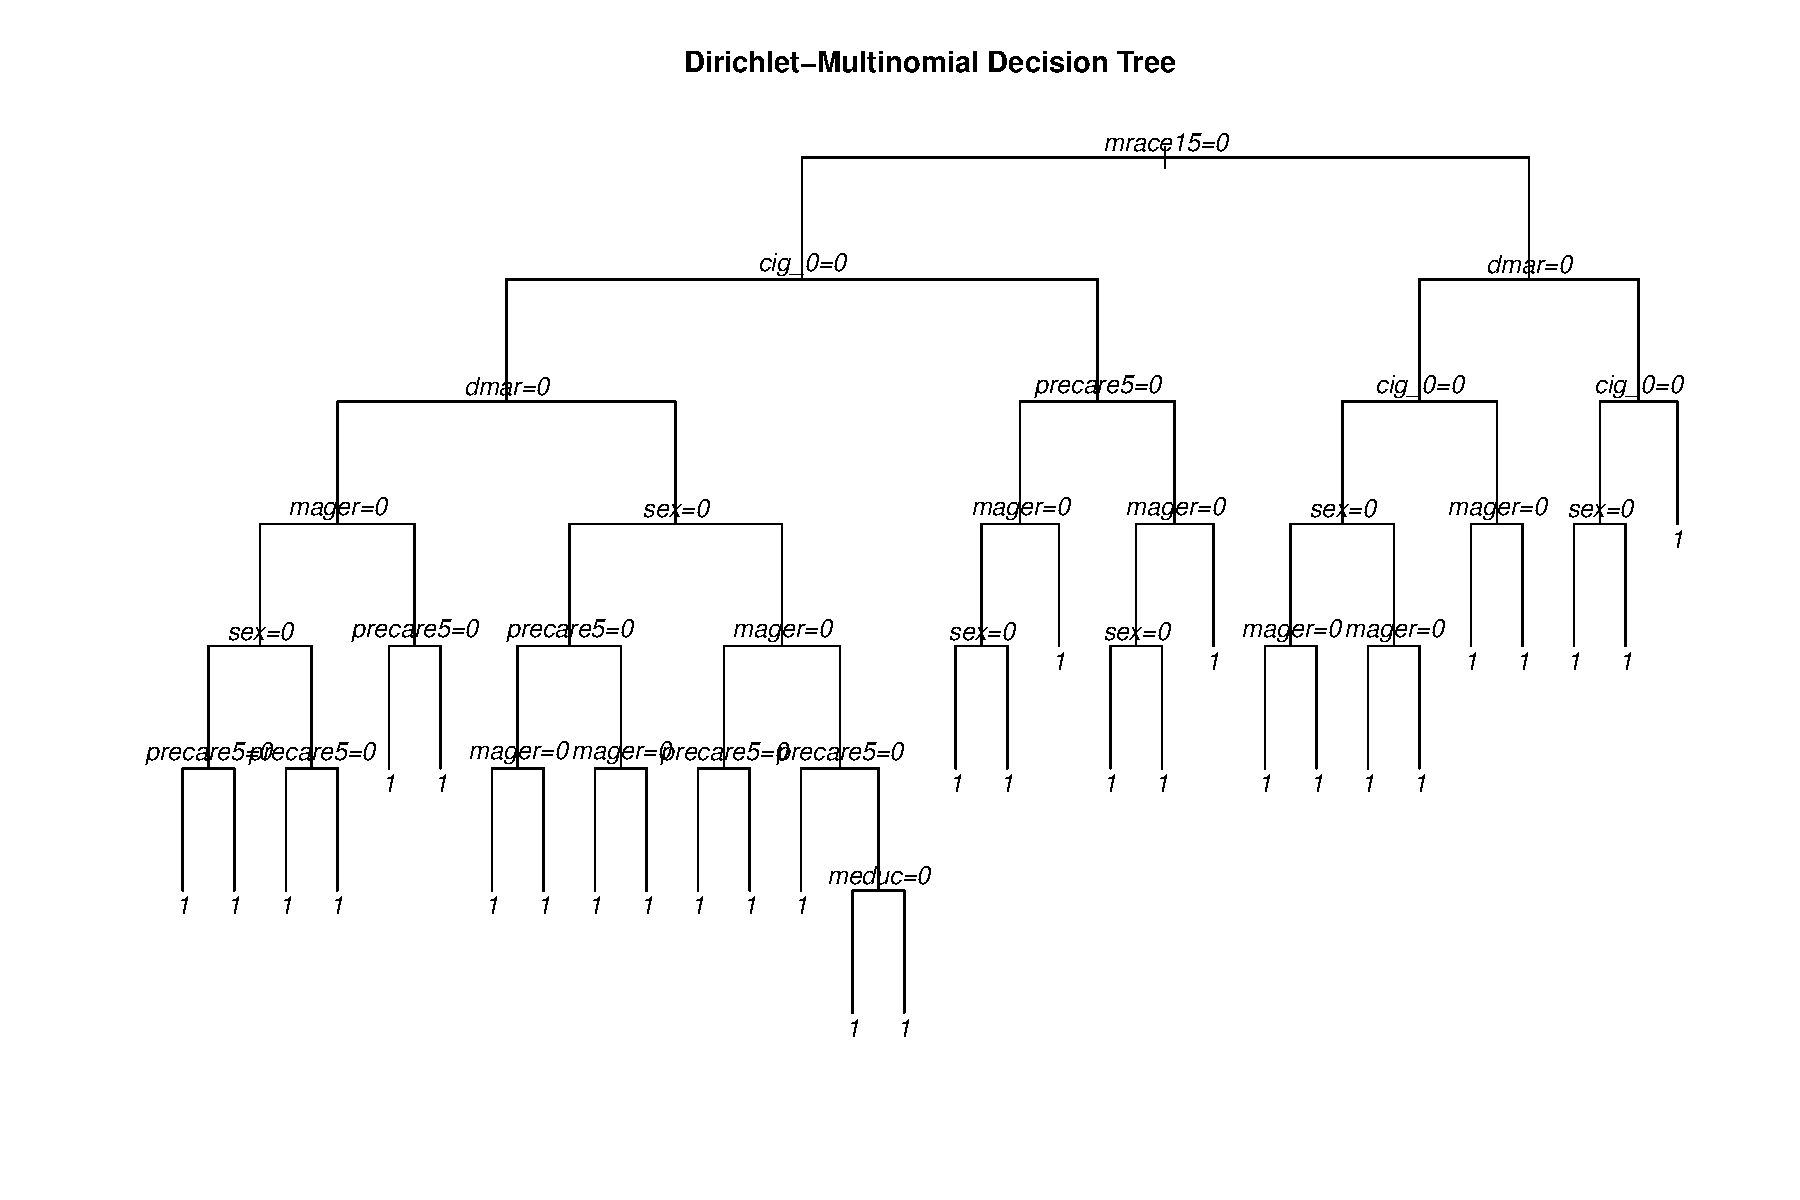
\includegraphics[width=\linewidth]{images/plots/dm_tree2021.pdf}\\[-0.8ex]
      {\small Full model}
    \end{minipage}\hfill
    \begin{minipage}{0.50\linewidth}
      \centering
      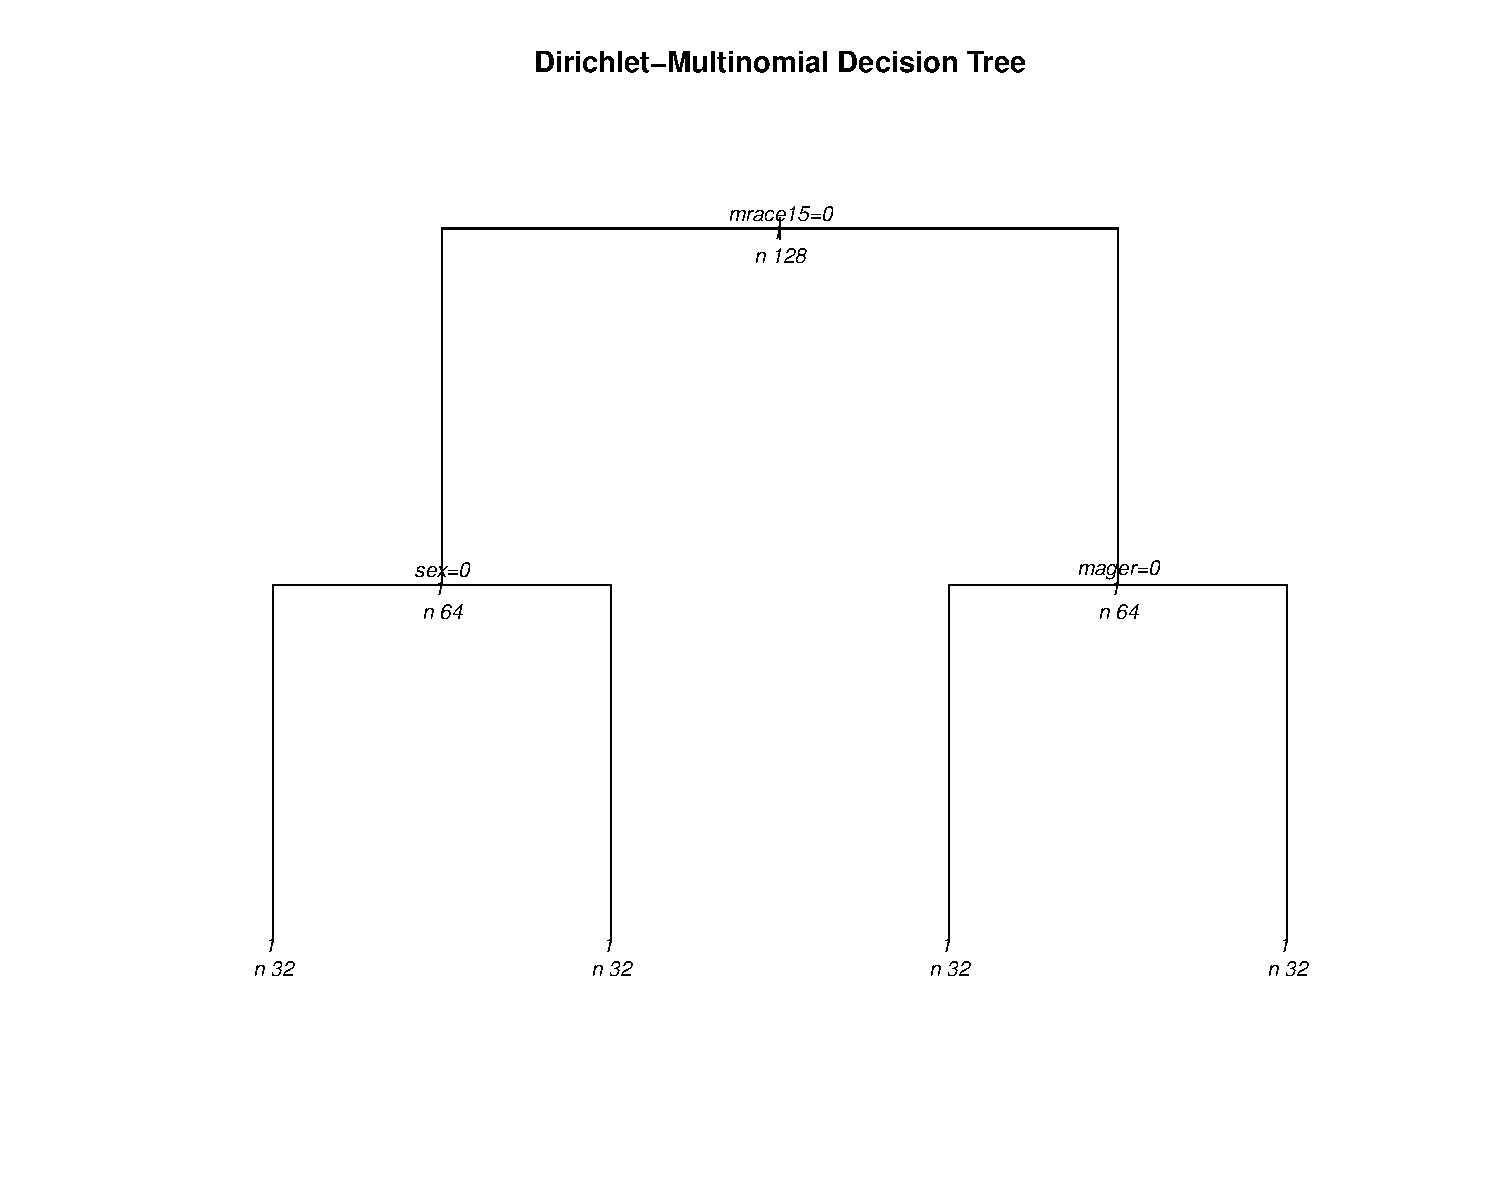
\includegraphics[width=\linewidth]{images/plots/dm_tree2021_2.pdf}\\[-2em]
      {\small LBW-only}
    \end{minipage}
    
    Using \texttt{rpart}  developed by \citet{breiman1984classification, rpart_docs}

    \textbf{Highlights:}\vspace{-0.4em}
    \begin{itemize}\tightlist
      \item \emph{Full model:} Root = race, then smoking, marital status predominantly. \emph{Socioeconomic focus.} 
      \item \emph{LBW-only:} Root = race, then infant sex, maternal age, prenatal care. \emph{Biological focus.}
    \end{itemize}
    
\end{alertblock}


\vspace{-1.5em}
\begin{block}{Two-Tier Bootstrap: Design and Implementation}
  
  Notation: \(T = \sum_i \sum_k n_{i,k}\) (grand total), \(p_i =  N_i / T\), \(\mathbf{p} = (p_1, \dots, p_N),\) (empirical class shares)

  Tier 1: \textbf{Between-class} counts resampling, propagating the prevalence of \(N\) profiles. 
  
  \(\mathbf{n}^\ast = (n_1^\ast, \dots, n_N^\ast) \sim \mathrm{Multinomial}(T,\mathbf{p})\). 
  
  Tier 2: \textbf{Within-class} counts resampling, for \(K\) category counts with \(n_i^\ast>0\)
  
  \(\tilde{\mathbf{y}}_i = (\tilde{n}_{i,1}, \dots, \tilde{n}_{i,K}) \sim \mathrm{Multinomial}(n_i^\ast,\hat{\boldsymbol{\pi}}_i)\), \quad (creating resampled response matrix: \(\tilde{\mathbf{Y}}\))
  
  where \(\hat{\pi}_{i,k}=(n_{i,k}+\alpha_k)/(N_i+\alpha_0)\) gives the mean bootstrap estimate for (\(i,k\)) (Table~\ref{tab:var-imp})

  \end{block}

\end{column}

\separatorcolumn

\begin{column}{\colwidth}
\vspace{-1em}
\begin{block}{Bootstrap Results: Variable Importance and Interpretation}
    \small
    \begin{minipage}[t]{0.45\linewidth}
      \raggedright
      {\bf Variable Importance}\par\vspace{1mm}
      \begin{tabular}{@{}lcc@{}}
        \toprule
                     & \multicolumn{1}{c}{\textbf{Full Model}} & \multicolumn{1}{c}{\textbf{LBW-Only Model}} \\
        \cmidrule(lr){2-2}\cmidrule(lr){3-3}
        \multicolumn{3}{l}{\emph{Initial Split Variable}} \\
        \midrule
        mrace15         & 1.0000 & 1.0000 \\
        \midrule
        \multicolumn{3}{l}{\emph{Variable Frequency}} \\
        \midrule
        sex             & 1.0000 & 1.0000 \\
        dmar            & 1.0000 & 0.0915 \\
        mrace15         & 1.0000 & 1.0000 \\
        mager           & 1.0000 & 0.9741 \\
        precare5        & 1.0000 & 0.6351 \\
        cig\_0          & 1.0000 & 0.0196 \\
        meduc           & 0.3794 & 0.0000 \\
        \bottomrule
        \label{tab:var-imp}
      \end{tabular}
    \end{minipage}\hfill
    \begin{minipage}[t]{0.50\linewidth}
      \raggedright
      % Vanilla LaTeX list with tight spacing and small left margin
      \begin{list}{\textbullet}{%
          \setlength{\leftmargin}{-4em}%
          \setlength{\labelsep}{0.4em}%
          \setlength{\itemsep}{0.7ex}%
          \setlength{\topsep}{0.2ex}%
          \setlength{\parsep}{0pt}%
      }
      \normalsize
        \item \textbf{Full model:} Race, smoking, marital status dominate; prenatal care and age enter later; education deep in 38\% of trees.
        \item \textbf{LBW-only:}  Race, sex, and age dominate; socioeconomic predictors mostly absent (<10\%).
        \item Confirms racial disparities as the most consistent and influential signal in LBW incidence.
        \item \emph{Context of data limits diverse BW outcomes and splits.}
        \item Variable inclusion percentages \emph{highlight the relative importance} of each, under different contexts.
      \end{list}
    \end{minipage}
    
\end{block}
\vspace{-2.4em}


\begin{block}

    Aggregate mean \(\hat{\pi}_{i,k}\) across \(B\) bootstraps with 95\% percentile intervals.

    \vspace{-.5em}

    \small
    \begin{itemize}\tightlist
        \item \emph{High-risk:} unmarried, Black, smoking mothers $<$33, $<$HS education, inadequate prenatal care, female infant.
        \item \emph{Low-risk:} married, non-Black, non-smoking mothers $\geq$33, $\geq$HS education, adequate prenatal care, male infant.
        \item For NBW, high-risk vs.\ low-risk prob. gap = 7\% (83.6\% vs.\ 90.9\%).
        \item In LBW region, extreme category risk can be \(3\times\) higher for high-risk.
    \end{itemize}
    
\begin{columns}[T]
  \column{0.50\linewidth}
    \centering
    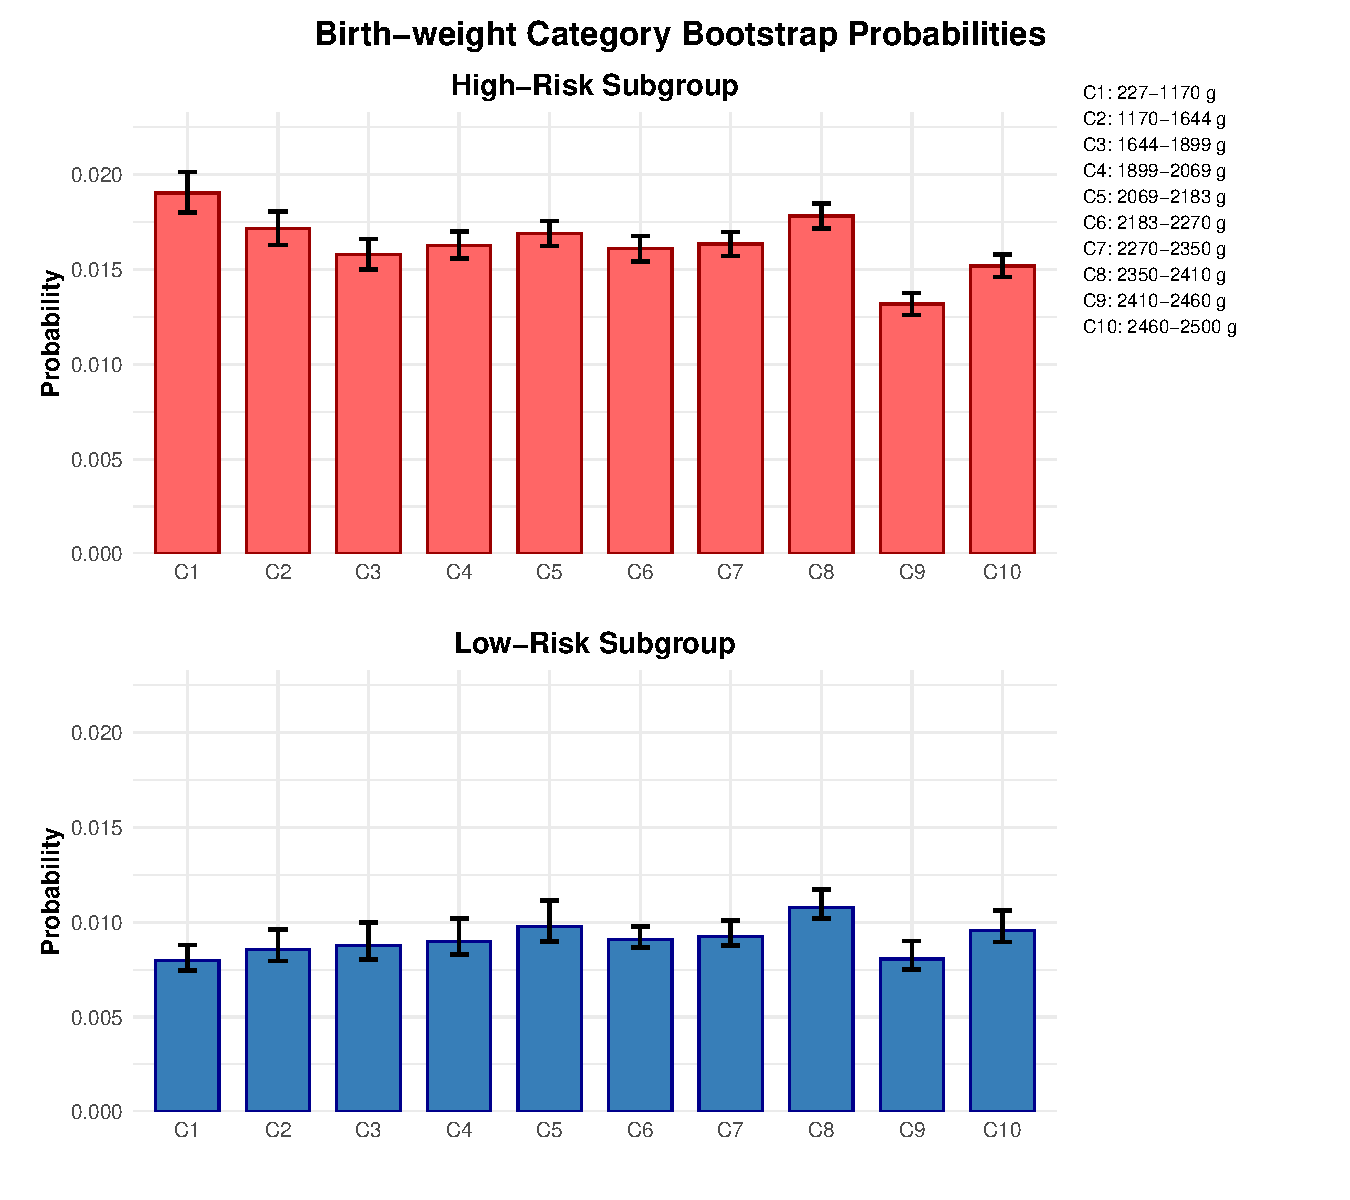
\includegraphics[width=\linewidth]{images/plots/high_low_risk_full_without_NBW.pdf}\\[-4pt]
    {\footnotesize Full model (no NBW): very narrow intervals ($\pm0.002$)}
  \column{0.50\linewidth}
    \centering
    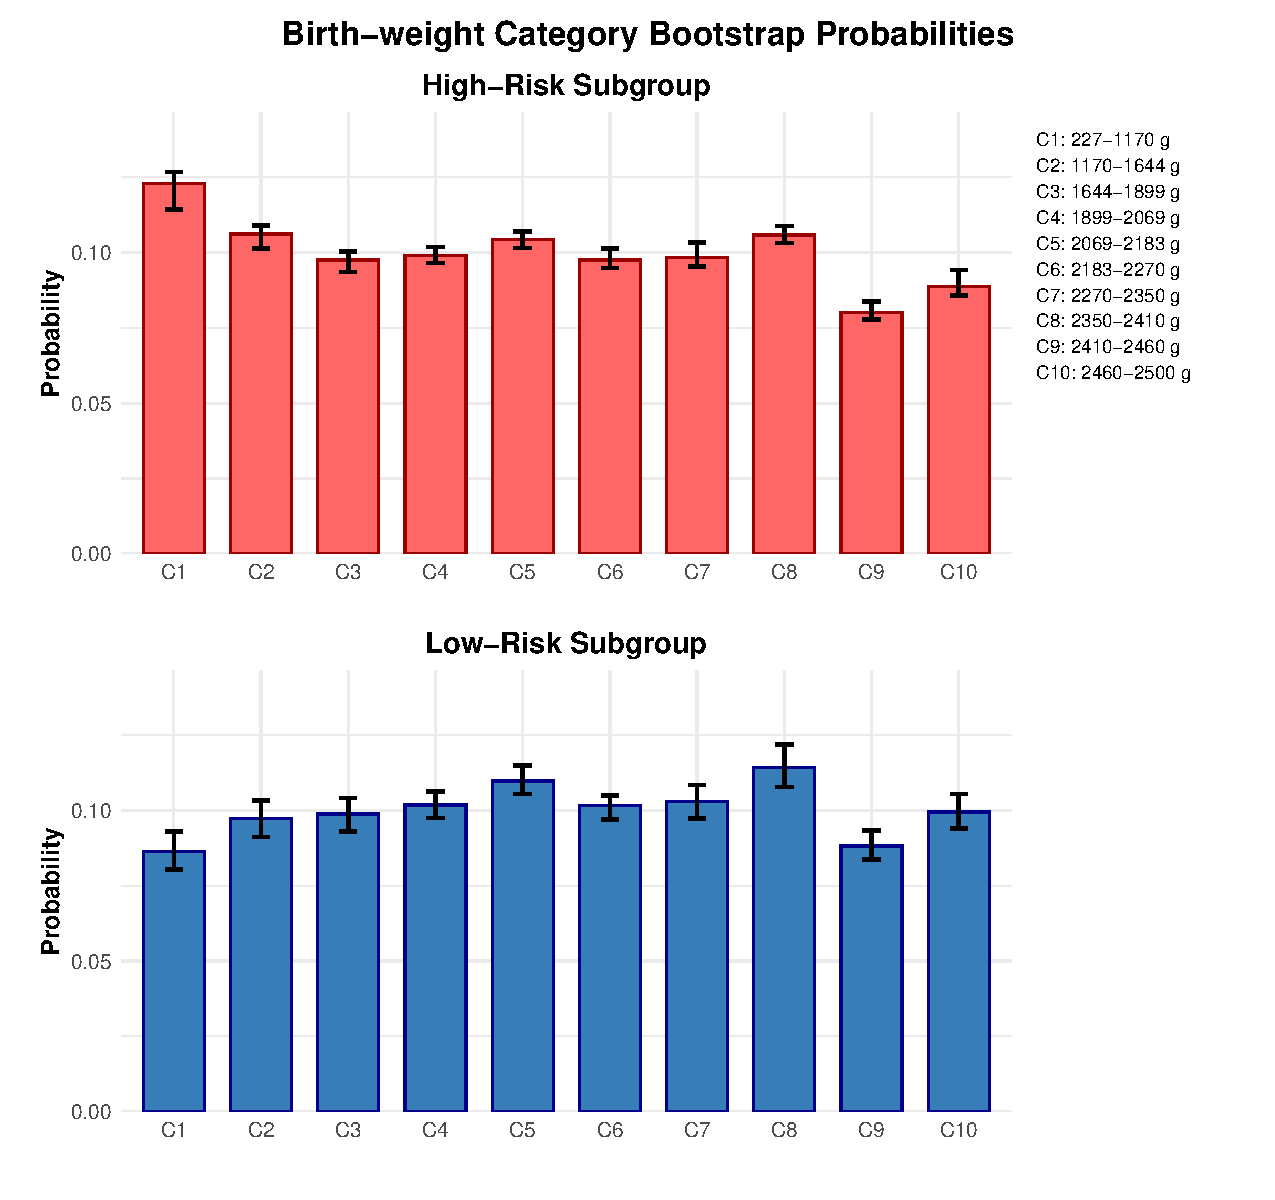
\includegraphics[width=\linewidth]{images/plots/high_low_risk_small.pdf}\\[-5pt]
    {\footnotesize LBW-only model: slightly wider intervals ($\pm0.008$)}
\end{columns}

  
\end{block}


\begin{alertblock}{Conclusions \& Future Work}          \vspace{-.4em}
    \small
    \begin{itemize}\tightlist
        \item \textbf{Model focus:} Full model uses socioeconomic and demographic information to contrast very diverse BW outcomes; LBW-only model identifies diversity within LBW region, biological predictors.
        \item \textbf{Key risk factors:} Maternal race, smoking, marital status; refined by infant sex, maternal age, prenatal care.
        \item \textbf{Performance:} DM-CART yields clear, epidemiologically consistent subgroup rules, stable across all bootstraps.
        \item\textbf{Future work:} Add richer maternal-health \& contextual variables, model multi-year trends, and explore clinical EHR integration.
    \end{itemize}
\end{alertblock}

\vspace{-1em}
\begin{block}{References}

    \tiny 
    \setlength{\bibsep}{0pt plus 0.3ex}
    \bibliographystyle{abbrv}\bibliography{poster}
    
  \end{block}

\end{column}

\separatorcolumn
\end{columns}
\end{frame}

\end{document}